\scanpage{60}
% archive sheet number: 59
\mspage{-VII- 19 -}\hfill n\textsuperscript{o}383

\uline{Système de racines de type} $G_2$

\figure{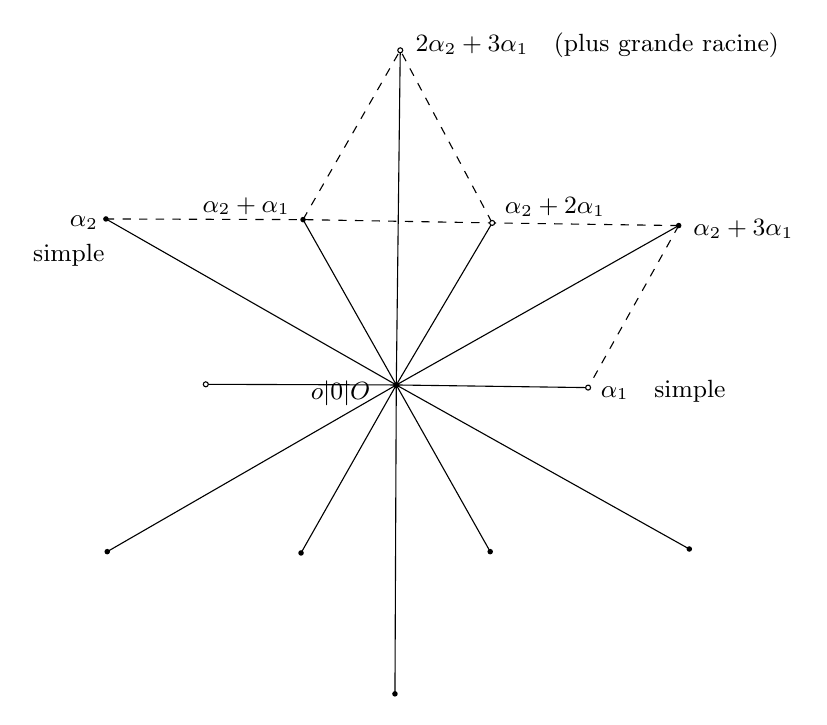
\begin{tikzpicture}[x=.84cm,y=.84cm,every node/.style={inner sep=2pt,font=\small}]
\coordinate (O) at (0,0);
\coordinate (T) at (.06,5.06);
\coordinate (NW) at (-4.39,2.51);
\coordinate (NNW) at (-1.41,2.50);
\coordinate (NNE) at (1.45,2.45);
\coordinate (NE) at (4.27,2.41);
\coordinate (E) at (2.90,-.04);
\coordinate (W) at (-2.88,.01);
\coordinate (SW) at (-4.37,-2.52);
\coordinate (SSW) at (-1.44,-2.54);
\coordinate (S) at (-.02,-4.67);
\coordinate (SSE) at (1.42,-2.52);
\coordinate (SE) at (4.43,-2.48);
\draw[dashed] (NW)--(NNW)--(NNE)--(NE);
\draw[dashed] (NNW)--(T)--(NNE);
\draw[dashed] (NE)--(E);
\draw (O)--(T) (O)--(NW) (O)--(NNW) (O)--(NNE) (O)--(NE) (O)--(E)
      (O)--(W) (O)--(SW) (O)--(SSW) (O)--(S) (O)--(SSE) (O)--(SE);
\fill (NW) circle (1pt) (NNW) circle (1pt) (NE) circle (1pt) (SW) circle (1pt)
      (SSW) circle (1pt) (S) circle (1pt) (SSE) circle (1pt) (SE) circle (1pt);
\draw[fill=white] (T) circle (.9pt) (NNE) circle (.9pt) (E) circle (.9pt) (W) circle (.9pt);
\node[anchor=west] at (.20,5.13) {$\handwritten{2\alpha_2+3\alpha_1}$\quad (plus grande racine)};
\node[anchor=east] at (-4.42,2.46) {$\handwritten{\alpha_2}$};
\node[anchor=north east] at (-4.32,2.22) {simple};
\node[anchor=south east] at (-1.52,2.48) {$\handwritten{\alpha_2+\alpha_1}$};
\node[anchor=south west] at (1.55,2.46) {$\handwritten{\alpha_2+2\alpha_1}$};
\node[anchor=west] at (4.40,2.36) {$\handwritten{\alpha_2+3\alpha_1}$};
\node[anchor=west] at (3.00,-.09) {$\handwritten{\alpha_1}$\quad simple};
\node[anchor=east] at (-.30,-.12) {$\handwritten{\unsure{o|0|O}}$};
\end{tikzpicture}}
